% Created 2022-11-07 Mon 16:04
% Intended LaTeX compiler: pdflatex
\documentclass[presentation,aspectratio=169]{beamer}
\usepackage[utf8]{inputenc}
\usepackage[T1]{fontenc}
\usepackage{graphicx}
\usepackage{grffile}
\usepackage{longtable}
\usepackage{wrapfig}
\usepackage{rotating}
\usepackage[normalem]{ulem}
\usepackage{amsmath}
\usepackage{textcomp}
\usepackage{amssymb}
\usepackage{capt-of}
\usepackage{hyperref}
\usepackage{khpreamble}
\usepackage{amssymb}
\usepackage{tcolorbox}
\usepackage{pgfplots}
\usepgfplotslibrary{groupplots}
\DeclareMathOperator{\shift}{q}
\DeclareMathOperator{\diff}{p}
\usetheme{default}
\author{Kjartan Halvorsen}
\date{\today}
\title{Stability}
\hypersetup{
 pdfauthor={Kjartan Halvorsen},
 pdftitle={Stability},
 pdfkeywords={},
 pdfsubject={},
 pdfcreator={Emacs 26.3 (Org mode 9.4.6)}, 
 pdflang={English}}
\begin{document}

\maketitle

\section{Intro}
\label{sec:orgf404d43}

\begin{frame}[label={sec:org3488c90}]{Hard disk drive arm model}
\begin{center}
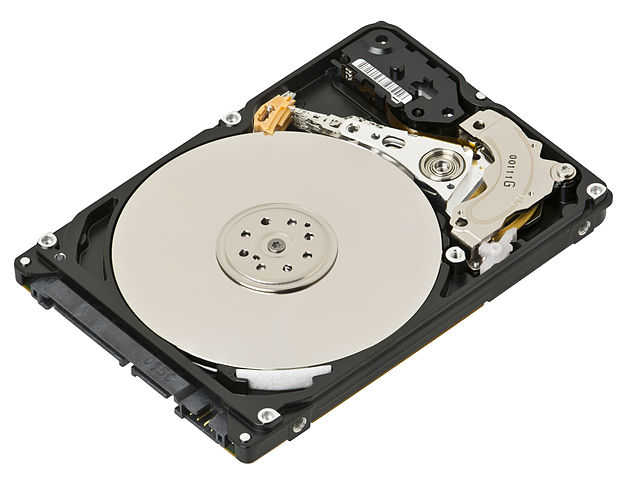
\includegraphics[width=0.4\linewidth]{../../figures/diskdrive.png}
\end{center}

{\tiny "Laptop-hard-drive-exposed" by Evan-Amos - Own work. Licensed under CC BY-SA 3.0 via Commons } 
\end{frame}

\begin{frame}[label={sec:org31d638f}]{Sampling the hard disk drive arm model}
\footnotesize
\[ H(z) = \frac{z-1}{z} \ztrf{\mathcal{L}^{-1}\{ \frac{G(s)}{s} \}} \]
\begin{center}
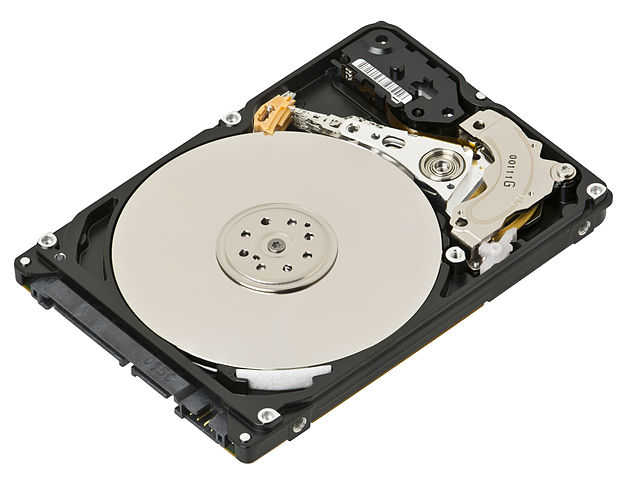
\includegraphics[height=0.25\textheight]{../../figures/diskdrive.png} 
\begin{tikzpicture}[scale=0.7, node distance=2.2cm, block/.style={rectangle, draw, minimum height=12mm, minimum width=12mm}, sumnode/.style={circle, draw, inner sep=1pt}]
\footnotesize
  \node[coordinate] (input) {};
  \node[block, right of=input] (plant) {$\frac{1}{Js^2}$};
  \node[coordinate, right of=plant] (output) {};
  \draw[->] (input) -- node[above] {$u$} (plant);
  \draw[->] (plant) -- node[above] {$y$} (output);

  \node at (-2, 1) {$J\ddot{y} = u$};
  \end{tikzpicture}
\end{center}

\pause

Which of the below graphs show the sampled \alert{step-response} of the system?

\begin{center}
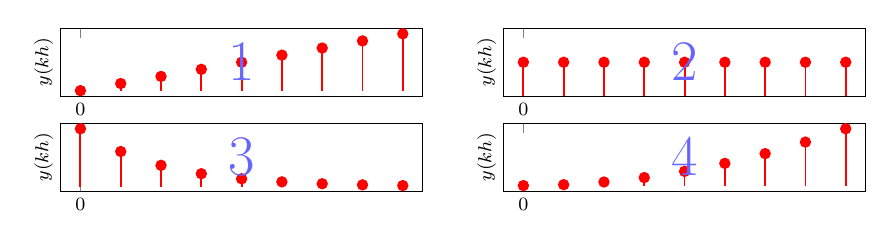
\begin{tikzpicture}[scale=0.85]
       \footnotesize

       \begin{groupplot}[group style={group size=2 by 2, vertical sep=1.2cm, horizontal sep=1.2cm, vertical sep=4mm},
       width=7cm,
       height=2.6cm,
       %xlabel={$t$},
       ylabel={$y(kh)$},
       xmin=-0.5,
       xmax=8.5,
       ytick = \empty,
       xtick = 0,
       ]
       \nextgroupplot
       \addplot[red, thick, ycomb, mark=*,domain=0:8, samples=9]  {x};

       \nextgroupplot
       \addplot[red, thick, ycomb, mark=*, domain=0:8, samples=9]  {1};

       \nextgroupplot
       \addplot[red, thick, ycomb, mark=*, domain=0:8, samples=9]  {2*exp(-x/2)};

       \nextgroupplot
       \addplot[red, thick, ycomb, mark=*,domain=0:8, samples=9]  {pow(x,2)};
       
     \end{groupplot}
     \node[blue!60] at (group c1r1.center) {\huge 1};
       \node[blue!60] at (group c2r1.center) {\huge 2};
       \node[blue!60] at (group c1r2.center) {\huge 3};
       \node[blue!60] at (group c2r2.center) {\huge 4};
       \end{tikzpicture}

     \end{center}
\end{frame}


\begin{frame}[label={sec:orgef15874}]{Sampling the hard disk drive arm model}
\footnotesize
\[ H(z) = \frac{z-1}{z} \ztrf{\mathcal{L}^{-1}\{ \frac{G(s)}{s} \}} \]
\begin{center}
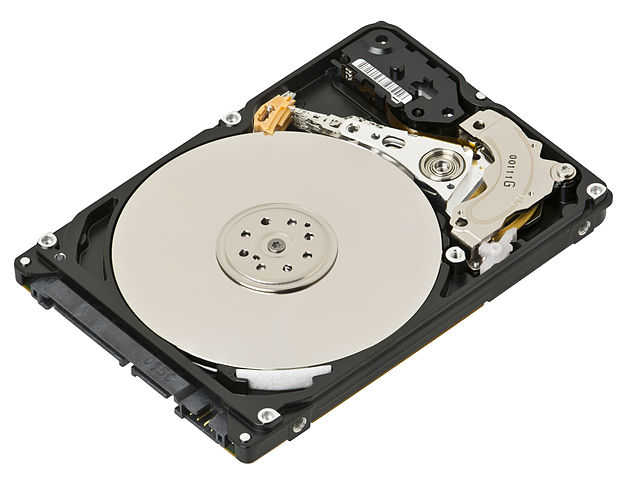
\includegraphics[height=0.25\textheight]{../../figures/diskdrive.png} 
\begin{tikzpicture}[scale=0.7, node distance=2.2cm, block/.style={rectangle, draw, minimum height=12mm, minimum width=12mm}, sumnode/.style={circle, draw, inner sep=1pt}]
\footnotesize
  \node[coordinate] (input) {};
  \node[block, right of=input] (plant) {$\frac{1}{Js^2}$};
  \node[coordinate, right of=plant] (output) {};
  \draw[->] (input) -- node[above] {$u$} (plant);
  \draw[->] (plant) -- node[above] {$y$} (output);

  \node at (-2, 1) {$J\ddot{y} = u$};
  \end{tikzpicture}
\end{center}

Sampled step-response: \(y(kh) = \frac{1}{2J}(kh)^2\)
\[ k^2 \qquad \overset{\mathcal{Z}}{\longleftrightarrow} \qquad \frac{z(z+1)}{(z-1)^3}\]

\pause

Which of the below pulse-transfer functions corresponds to the discretized hard disk drive model?
\begin{center}
\begin{tabular}{rrr}
1 & 2 & 3\\
\(H(z)=\frac{h^2z}{2J(z+1)^2}\) & \(H(z)=\frac{h^2(z+1)}{2Jz^2}\) & \(H(z)=\frac{h^2(z+1)}{2J(z-1)^2}\)\\
\end{tabular}
\end{center}
\end{frame}

\section{Block-diagram algebra}
\label{sec:org565138f}
\begin{frame}[label={sec:orge97b493}]{Block-diagram algebra}
\alert{Same rules as in the continuous-time case!}
\begin{center}
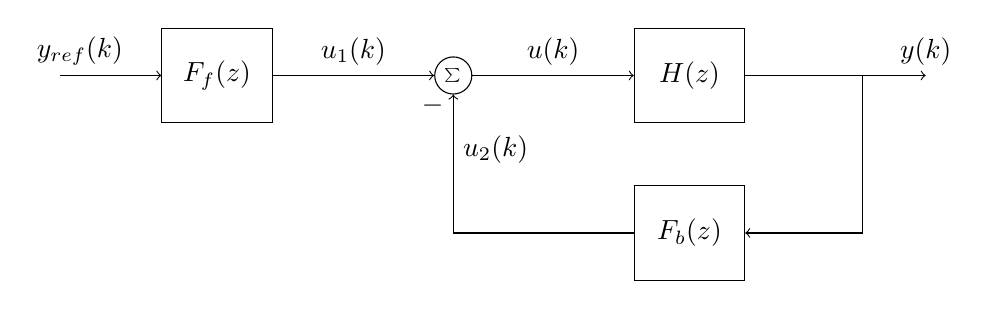
\begin{tikzpicture}
\tikzset{node distance=2cm, 
    block/.style={rectangle, draw, minimum height=12mm, minimum width=14mm},
    sumnode/.style={circle, draw, inner sep=2pt}        
}

  \node[coordinate] (input) {};
  \node[block, right of=input] (TR) {$F_f(z)$};
  \node[sumnode, right of=TR, node distance=30mm] (sum) {\tiny $\sum$};
  \node[block,right of=sum, node distance=30mm] (plant) {$H(z)$};
  %\node[sumnode, right of=plant, node distance=30mm] (sumdist) {$\sum$};
  %\node[coordinate, above of=sumdist, node distance=15mm] (dist) {};
  %\node[coordinate, right of=sumdist, node distance=15mm] (measure) {};
  \node[coordinate, right of=plant, node distance=30mm] (output) {};
  \node[coordinate, right of=plant, node distance=22mm] (measure) {};
  %\node[sumnode,below of=measure, node distance=25mm] (sumnoise) {$\sum$};
  %\node[coordinate, right of=sumnoise, node distance=15mm] (noise) {};
  \node[block,below of=plant, node distance=20mm] (SR) {$F_b(z)$};
  \draw[->] (input) -- node[above, pos=0.2] {$y_{ref}(k)$} (TR);
  \draw[->] (TR) -- node[above] {$u_1(k)$} (sum);
  \draw[->] (sum) -- node[above] {$u(k)$} (plant);
  \draw[->] (plant) -- node[at end, above] {$y(k)$} (output);
  \draw[->] (measure) |- (SR);
  \draw[->] (SR) -| (sum) node[right, pos=0.8] {$u_2(k)$} node[left, pos=0.96] {$-$};
\end{tikzpicture}
\end{center}
With \[U(z) = U_1(z) - U_2(z) = F_f(z)Y_{ref}(z) - F_b(z)Y(z), \quad \text{and}\]
\[ Y(z) = H(z)U(z), \quad \text{we obtain} \]
\[ Y(z) = \underbrace{\frac{F_f(z)H(z)}{1 + F_b(z)H(z)}}_{H_c{z}} Y_{ref}(z). \]
\end{frame}

\begin{frame}[label={sec:orgd60d324}]{Block-diagram algebra - steps in detail}
With \[U(z) = U_1(z) - U_2(z) = F_f(z)Y_{ref}(z) - F_b(z)Y(z), \quad \text{and}\]
\[ Y(z) = H(z)U(z), \quad \text{we obtain} \]
\[ Y(z) = H(z)U(z) = H(z)\left(F_f(z)Y_{ref}(z) - F_b(z)Y(z)\right)\]
Move all terms with \(Y\) to the left side:
\[ Y(z) + H(z)F_b(z)Y(z) = H(z)F_f(z)Y_{ref}(z)\]
\[ Y(z)\big(1 + H(z)F_b(z)\big) = H(z)F_f(z)Y_{ref}(z)\]
\[ Y(z) = \frac{H(z)F_f(z)}{1 + H(z)F_b(z)}Y_{ref}(z)\]
\end{frame}

\begin{frame}[label={sec:org439e8ac}]{Stability for the closed-loop system}
\[ Y(z) = \frac{F_f(z)H(z)}{1 + F_b(z)H(z)} Y_{ref}(z). \]

\begin{tcolorbox}
Stability requires that all poles of the system, i.e. all solutions to the characteristic equation
\[ 1 + F_b(z)H(z) = 0\]
are located inside the unit circle of the  z-plane.
\end{tcolorbox}
\end{frame}

\begin{frame}[label={sec:org0f15104}]{Stability for the disk drive arm}
\small 
Case \(\frac{h^2}{J} = 1\). Suggested controller:

\begin{center}
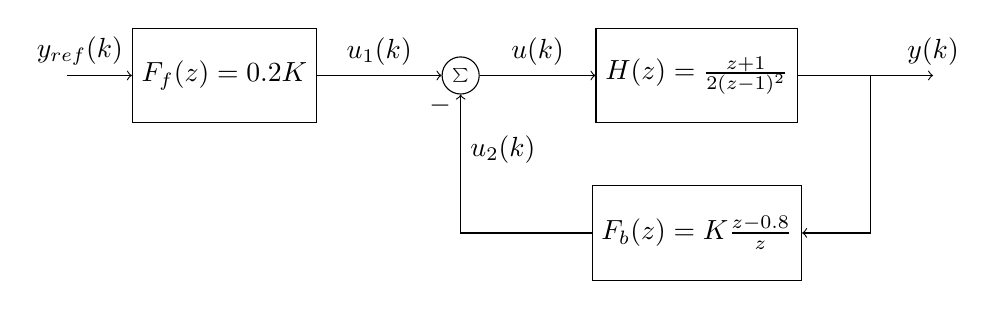
\begin{tikzpicture}
\tikzset{node distance=2cm, 
    block/.style={rectangle, draw, minimum height=12mm, minimum width=14mm},
    sumnode/.style={circle, draw, inner sep=2pt}        
}

  \node[coordinate] (input) {};
  \node[block, right of=input] (TR) {$F_f(z) = 0.2K$};
  \node[sumnode, right of=TR, node distance=30mm] (sum) {\tiny $\sum$};
  \node[block,right of=sum, node distance=30mm] (plant) {$H(z) = \frac{z+1}{2(z-1)^2}$};
  %\node[sumnode, right of=plant, node distance=30mm] (sumdist) {$\sum$};
  %\node[coordinate, above of=sumdist, node distance=15mm] (dist) {};
  %\node[coordinate, right of=sumdist, node distance=15mm] (measure) {};
  \node[coordinate, right of=plant, node distance=30mm] (output) {};
  \node[coordinate, right of=plant, node distance=22mm] (measure) {};
  %\node[sumnode,below of=measure, node distance=25mm] (sumnoise) {$\sum$};
  %\node[coordinate, right of=sumnoise, node distance=15mm] (noise) {};
  \node[block,below of=plant, node distance=20mm] (SR) {$F_b(z)=K\frac{z-0.8}{z}$};
  \draw[->] (input) -- node[above, pos=0.2] {$y_{ref}(k)$} (TR);
  \draw[->] (TR) -- node[above] {$u_1(k)$} (sum);
  \draw[->] (sum) -- node[above] {$u(k)$} (plant);
  \draw[->] (plant) -- node[at end, above] {$y(k)$} (output);
  \draw[->] (measure) |- (SR);
  \draw[->] (SR) -| (sum) node[right, pos=0.8] {$u_2(k)$} node[left, pos=0.96] {$-$};
\end{tikzpicture}
\end{center}

\alert{Characteristic equation}
\begin{align*}
1 + H(z)F_b(z) &= 0\\
1 + \frac{z+1}{2(z-1)^2}K\frac{z-0.8}{z} &= 0\\
(z-1)^2z + \frac{K}{2}(z+1)(z-0.8) &= 0
\end{align*}

\pause

\alert{Is the system stable for all gains \(K\)?}
\end{frame}


\begin{frame}[label={sec:orgae90d3a}]{Stability for the disk drive arm}
\alert{Pair activity} Complete the root-locus below

\[(z-1)^2z + \frac{K}{2}(z+1)(z-0.8) = 0\]
\begin{center}
  \begin{tikzpicture}[scale=2.5]
    \draw[->] (-1.2, 0) -- (1.2,0);
    \draw[->] (0, -1.2) -- (0,1.2);
    \node[red, pin=45:{2 plant poles}] at (1,0) {\large $\times$};
    \node[red, pin=135:{controller pole}] at (0,0) {\large $\times$};
    \node[green!70!black, pin=-145:{controller zero}] at (0.8,0) {\Large $\circ$};
    \node[green!70!black, pin=-145:{plant cero}] at (-1,0) {\Large $\circ$};
    \node at (0.8, -0.2) {$0.8$};
    \node at (1, -0.2) {$1$};
    \draw[domain=0:360, samples=361, dashed] plot ({cos(\x)}, {sin(\x)});
    \node[coordinate, pin=60:{$|z|=1$}] at (0.5, 0.87) {};
  \end{tikzpicture}
\end{center}
\end{frame}


\section{Estabilidad para el control del brazo del disko duro}
\label{sec:org8122e64}
\end{document}